\documentclass{acmtog}

\begin{document}
\title{ACTIVE LEARNING IN TEXT CLASSIFICATION} % title
\author{YUYI GU {\upshape and} LINGJIA LI
\affil{Shanghai Jiao Tong University}}

\maketitle

\begin{abstract}
In many real-world domains, supervised learning requires a large number of training examples. In this paper, we describe an active learning method that is classifier-agnostic and we have shown that it works across classifiers and feature representations. Our approach is similar to uncertainty sampling, where data with the least probability difference between the classifier giving the two most probable labels is queried. Our experiments are conducted in the text classification domain, which is characterized by a large number of features, many of which are irrelevant.
 
\end{abstract}

\section{Introduction}
The goal of\textit{ text classification }is to assign each document to the appropriate categories, based on the semantic content of the document. A knowledge engineering approach to text classification involves designing rules that correctly classify the documents. The goal is to develop \textbf{automatic} methods for text classification through the application of machine learning techniques.
The amount of textual information that is available in electronic form has grown exponentially in recent years. Annotating documents for supervised learning has been a tedious, laborious, and time consuming task for humans. Given huge amounts of unlabeled documents, it is impractical for annotators to go over each document and provide a label. Automating the task of indexing, categorizing, and organizing these electronic documents will make it easier and cheaper for people to find relevant written materials.

\textit{Active learning} refers to machine learning methods that allow the learning program to exert some control over the examples on which it learns \cite{cohn1994improving}. The purpose of this paper is to present results of experiments that demonstrate the effectiveness of active learning with uncertainty sampling, and also to analyze the sources of this effectiveness. 

\section{Related Work }
\label{sec:relatedwork}
Active learning has long been a popular field that many researchers have contributed to it. 
"Active learning" in its most general sense refers to any form of learning where in the learning algorithm has some degree of control over the examples on which it is trained. One active learning approach is the membership query paradigm, in which the learner can construct new sets of inputs and request that the teacher provide their labels \cite{liere1997active}. 
There have been some promising results in the active learning area. Cohn, Atlas, and Ladner developed the theory for an active learning method called selective sampling and then applied it to some small to moderate sized problems as a demonstration of the viability of this new approach\cite{cohn1994improving}. Lewis and Gale developed a method called uncertainty sampling, which is similar conceptually to selective sampling, but which is specifically meant for use in text categorization. Their method selects for labeling those examples whose membership is most unclear by using an approximation based on Bayes Rule, certain independence assumptions, and logistic regression. Since the method was developed for text categorization, it is able to handle noise as well as large numbers of features\cite{lewis1994sequential}.

Dagan and Engelson use QBC stream-based sampling and vote entropy. In contrast, Andrew Kachites McCallumz et al. advocated density-weighted pool-based sampling and the KL metric.\cite{mccallumzy1998employing}  They selected committee
members using the Dirichlet distribution over classifier parameters, instead of approximating this with a Normal distribution. 


% One of the bottlenecks in eliciting domain knowledge from annotators is that the traditional supervised learning approaches cannot readily handle the elicited rich feedback. To address this issue, many methods have been developed that are classifier-specific. Examples include knowledge-based neural networks (e.g., (Towell and Shavlik, 1994), (Girosi and Chan, 1995), (Towell et al., 1990)), knowledge-based support vector machines (Fung et al., 2002), pooling multinomial na ̈ıve Bayes (Melville and Sindhwani, 2009), incorporating constraints into the training of näıve Bayes (Stumpf et al., 2007), and converting rationales and feature annotations into constraints for support vector machines (e.g., (Small et al., 2011) and (Zaidan et al., 2007)). 
%  Recent work on active learning with instance and feature annotations (e.g., (Melville and Sindhwani, 2009), (Druck et al., 2009), (Small et al., 2011), (Stumpf et al., 2008), (Raghavan and Allan, 2007), and (Attenberg et al., 2010)). 

 Manali Sharma et al.(2015) present a simple and yet effective active learning approach that can incorporate rationales elicited from annotators into the training of any off-the-shelf classifier\cite{sharma:naaclhlt15}. They show that their simple approach is effective for multinomial naive bayes, logistic regression, and support vector machines. 


\section{Brief Overview of ACTIVE LEARNING}
\label{sec:brifoverview}
\begin{figure*}[t]
\centerline{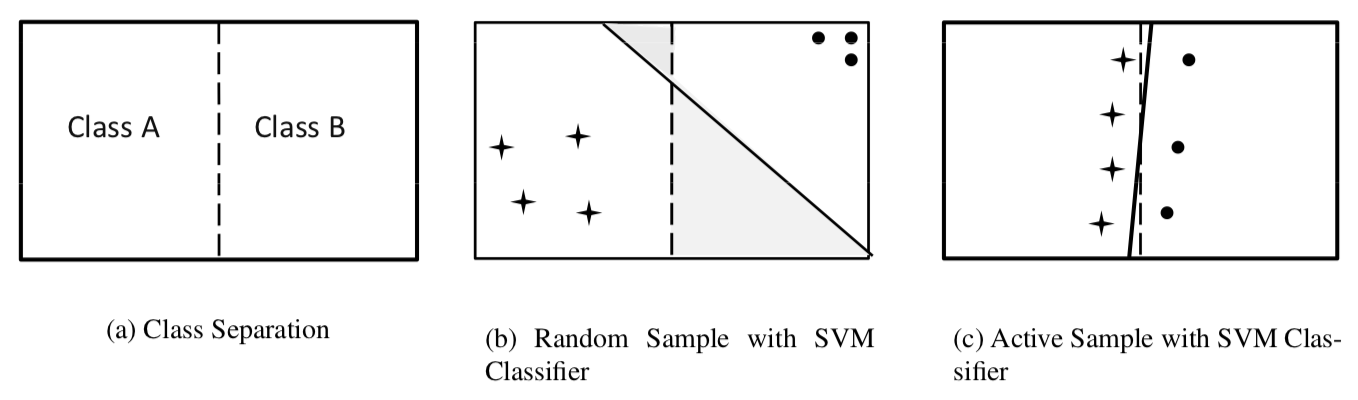
\includegraphics[width=11cm]{motivation}}
\caption{Motivation of active learning.}
  \label{fig:motivation}
\end{figure*}
Active learning (sometimes called “query learning” or “optimal experimental design” in the statistics literature) is a sub field of machine learning and, more generally, artificial intelligence. The key hypothesis is that if the learning algorithm is allowed to choose the data from which it learns to be “curious,” if you will, it will perform better with less training. 

While it is possible to query the data randomly for labels, such an approach may not result in the best model, when each query is costly, and therefore, few labels will eventually become available. For example, consider the two class example of Figure~\ref{fig:motivation}. Here, we have a very simple division of the data into two classes, which is shown by a vertical dotted line, as illustrated in Figure~\ref{fig:motivation}(a). The two classes here are labeled A and B. Consider the case where it is possible to query only 7 examples for the two different classes. In this case, it is quite possible that the small number of allowed samples may result in a training data that is unrepresentative of the true separation between the two classes. Consider the case when an SVM classifier is used in order to construct a model. In Figure~\ref{fig:motivation}(b), we have shown a total of 7 samples randomly chosen from the underlying data. Because of the inherent noisiness in the process of picking a small number of samples, an SVM classifier will be unable to accurately divide the data space. This is shown in Figure~\ref{fig:motivation}(b), where a portion of the data space is incorrectly classified, because of the error of modeling the SVM classifier. In Figure~\ref{fig:motivation}(c), we have shown an example of a well chosen set of seven instances along the decision boundary of the two classes. In this case, the SVM classifier is able to accurately model the decision regions between the two classes. This is because of the careful choice of the instances chosen by the active learning process. An important point to note is that it is particularly useful to sample instances that provide a distinct view of how the different classes are separated in the data.

\section{Problem Formulation}
\label{sub:problem_formulation}

\begin{figure}[t]
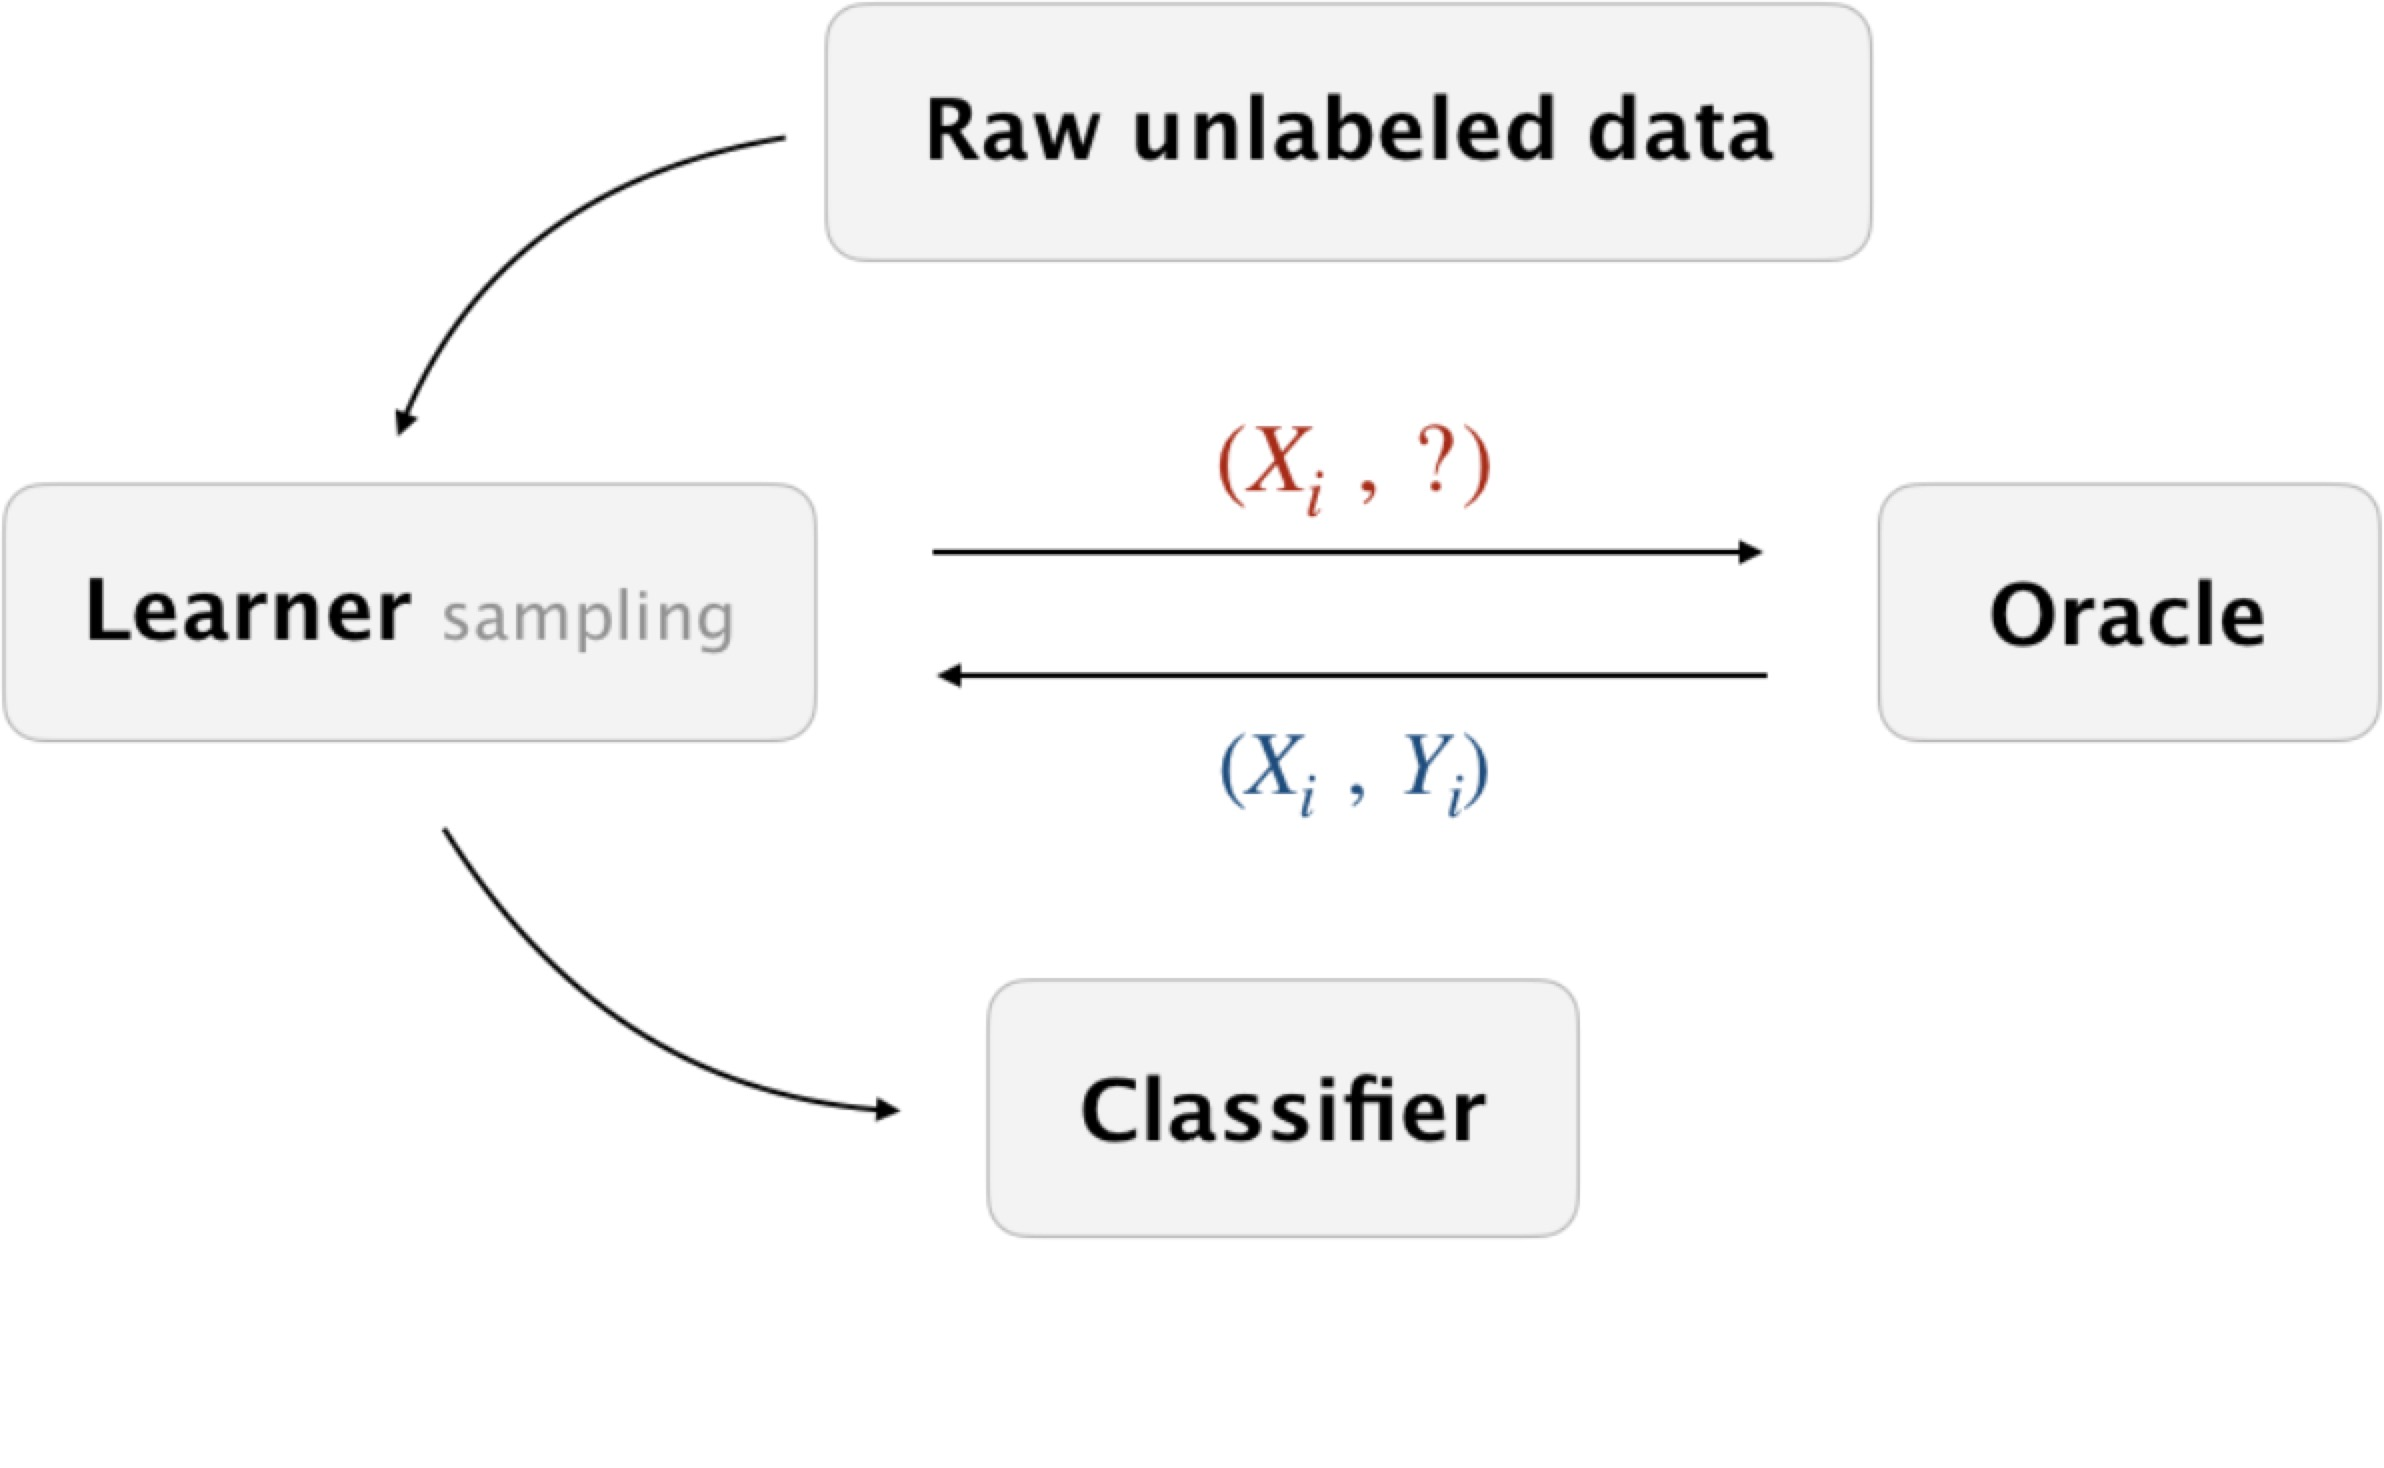
\includegraphics[width=8cm]{procedure}
\centering
\caption{Overall procedure in Active Learning}
  \label{fig:procedure}
\end{figure}
\begin{figure*}
\centering
\subfigure{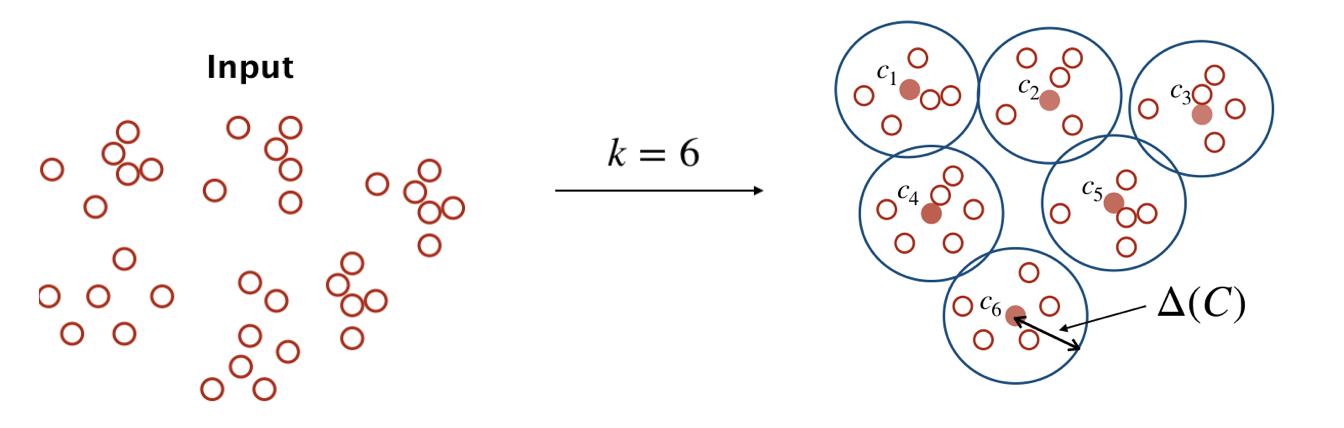
\includegraphics[width=12cm, angle=0]{kmeans1}}
\subfigure{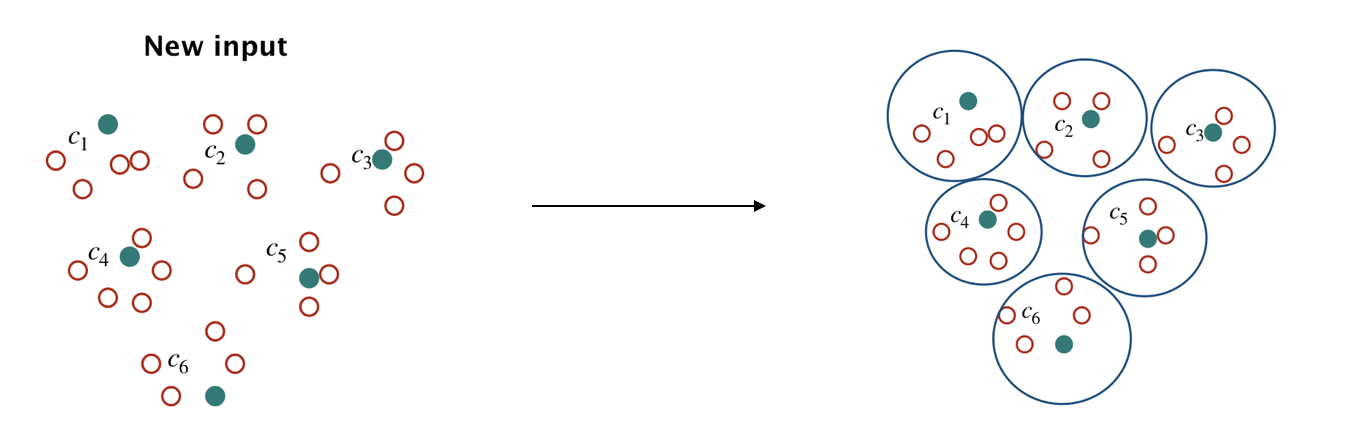
\includegraphics[width=12cm, angle=0]{kmeans2}}
\caption{Brief illustration on the procedure of K-center sampling ($k=6$)}
\label{fig:kmeans}
\end{figure*}

Let $D$ be a set of document-label pairs $(x,y)$, where the label (value of $y$) is known only for a small subset $L \subset D$ of the documents: $L = \{(x,y)\}$ and the rest $U=D \setminus L$ consists of the unlabeled documents: $U = \{(x, ?)\}$. We assume that each document $x_i$ is represented as a vector of features (most commonly as a bag-of-words model with a dictionary of predefined set of phrases, which can be unigrams, bigrams, etc.): 
\begin{eqnarray}
x_i \triangleq \{f_1^i,f_2^i,...,f_n^i\}
\end{eqnarray}
Each feature $f_j^i$ represents the binary presence (or absence), frequency, or tf-idf representation of the word/phrase $j$ in document $x^i$. Each label $y \in Y$ is discrete-valued variable 
\begin{eqnarray}
Y \triangleq \{y_1,y_2,...y_l\}
\end{eqnarray}
Typical greedy active learning algorithms iteratively select a document $(x, ?) \in  U$ , query a labeler for its label $y$, and incorporate the new document $(x, y)$ into its training set L. This process continues until a stopping criterion is met, usually until a given budget, B, is exhausted.

So the procedure of active learning, as is illustrated in Figure\ref{fig:procedure}, is first given some raw data, then the learner samples the point by  a certain criteria, and asks the oracle of the label, then feeds the labelled data back to the classifier.  After that, the classifier determines the decision boundary according to the given data.
\section{Proposed Methods}
\label{sec:proposed_methods}
The key question in active learning algorithms is to design the precise strategies that are used for querying. At any given point, our goal is to select sample so as to \textbf{maximize the accuracy} of the classification process. As is evident from the discussion in the previous section, it is advantageous to use strategies, so that the contours of separation between the different classes are mapped out with the use of a small number of examples. Since the boundary regions are often those in which instances of multiple classes are present, they can be characterized by class label uncertainty or disagreements between different learners. However, this may not always be the case, because instances with greater uncertainty are not representative of the data, and may sometimes lead to the selection
of unrepresentative outliers. This situation is especially likely to occur in data sets that are very noisy. In order to address such issues, some models focus directly on the error itself, or try to find samples that are representative of the underlying data. Therefore, we briefly introduce two types of models, heterogeneity and representativeness-based models.
\subsection{Heterogeneity Models}
\ \ \ \ Heterogeneity-based models\cite{aggarwal2014data} attempt to sample from regions of the space that are either more heterogeneous, or dissimilar to what has already been seen so far. Examples of such models include uncertainty sampling, query-by-committee, and expected model change. All these methods are based on sampling either uncertain regions of the data, or those that are dissimilar to what has been queried so far. These models not only look at the heterogeneity behavior of the queried instance, but also the effect of its addition on the performance of a classifier on the remaining unlabeled instances.
\subsubsection{Uncertainty Sampling}
The simplest and most commonly used query framework is uncertainty sampling. In this framework, the learner attempts to label those instances for which it is least certain how to label. 
The criteria is especially relevant for k-ary classification. It is the entropy measure or the gini-index. 
\begin{eqnarray}
G (\overline{X}) = 1-\sum_{i=1}^k {p_i}^2 
\end{eqnarray}
If the predicted probabilities of the k classes are $\{p_1,...,p_k\}$, respectively, based on the current set of labeled instances, then the entropy measure $En(\overline{X})$ is defined as follows:
\begin{eqnarray}
En(\overline{X}) = − \sum_{i=1}^k p_i log(p_i)
\end{eqnarray}
Larger values of the entropy indicate greater uncertainty. Therefore, this objective function needs to be maximized. 

\subsubsection{Margin-based Sampling}
We have found that the criterion for the least confident strategy only considers information about the most probable label. Thus, it effectively “throws away” information about the remaining label distribution. To correct for this, a different multi-class uncertainty sampling variant called\textit{ margin-based sampling} has been used.
\begin{eqnarray}
x^{*}_M =argmin_xP_{\theta}(\hat{y_1}|x)-P_{\theta}(\hat{y_2}|x)
\end{eqnarray}
where $\hat{y_1}$ and $\hat{y_2}$ are the first and second most probable class labels under the model, respectively. Margin-based sampling aims to correct for a shortcoming in least confident strategy, by incorporating the posterior of the second most likely la- bel. 
\subsection{Representativeness-Based Models}
Representativeness-based models attempt to create data that is as representative as possible of the underlying population of training instances. For example, density-based models are an example of such scenarios. In these cases, a product of a heterogeneity criterion and a representativeness criterion is used in order to model the desirability of querying a particular instance. Thus, these methods try to balance the representativeness criteria with the uncertainty properties of the queried instance.


As is shown in the exploded graph Figure~\ref{fig:kmeans}, if every time the learner will choose, let’s say, 6 points to query.  This algorithm will set k equal to 6 and performs the k-center greedy algorithm. After 6 points have been selected, the unlabeled data us removed, and  procedure is repeated. During the whole process, we only feed the data to the classifier, instead of asking the classifier its preference of data. 
\subsubsection{Hierarchical Sampling}
A hierarchical clustering of the unlabeled points is constructed so that some pruning of it is weakly informative of the class labels. Suppose it is possible to prune the cluster tree to m leaves (m unknown) that are fairly pure in the labels of their constituent points. Then, after querying just O(m) labels, the learner will have a fairly accurate estimate of the labels of the \textit{entire} data set. 

\section{Experiments}
\begin{figure}[t]
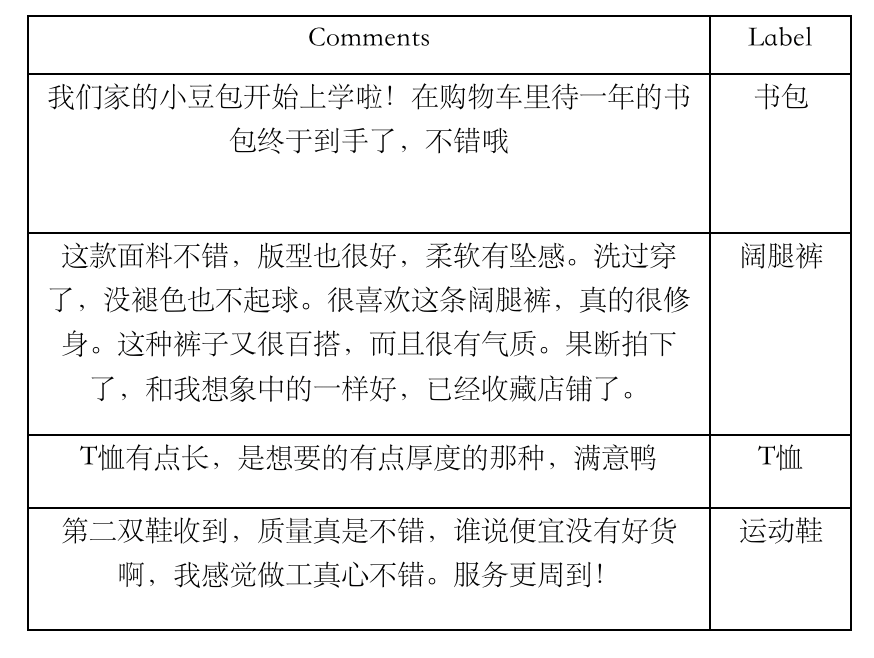
\includegraphics[width=8cm]{tbdb}
\centering
\caption{Taobao review}
  \label{fig:tbdb}
\end{figure}
\begin{figure}[t]
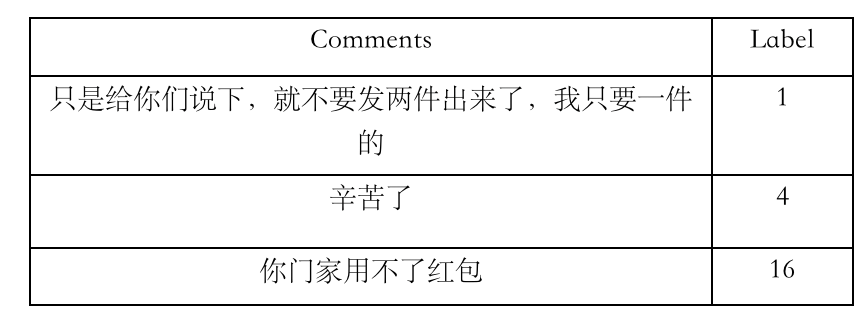
\includegraphics[width=8cm]{ecdb}
\centering
\caption{E-commerce customer queries}
  \label{fig:ecdb}
\end{figure}

\begin{figure*}
\centering
\subfigure{
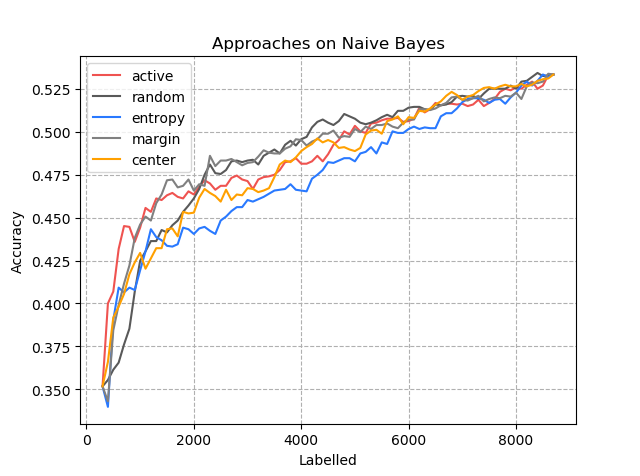
\includegraphics[width=5.5cm, angle=0]{tb1}
}
\subfigure{
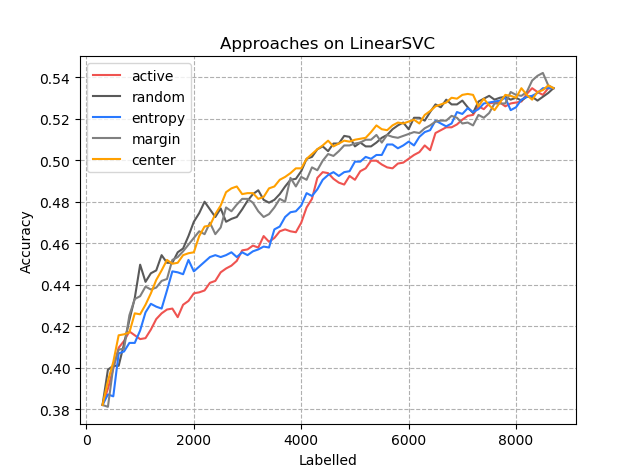
\includegraphics[width=5.5cm, angle=0]{tb2}
}
\subfigure{
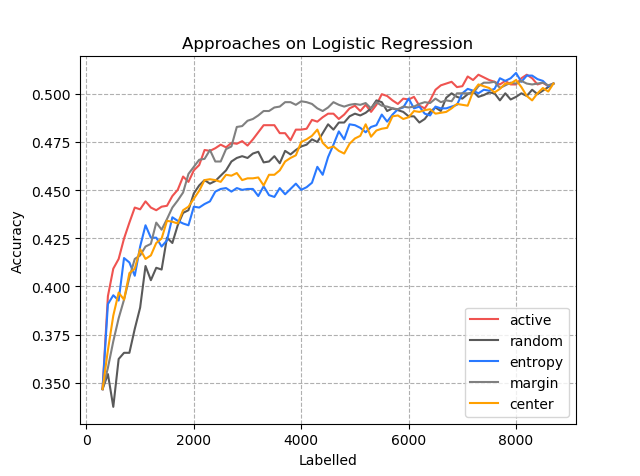
\includegraphics[width=5.5cm, angle=0]{tb3}
}
\caption{Results on Taobao review data set}
\label{fig:tb}
\end{figure*}

\begin{figure*}
\centering% Requires \usepackage{graphicx}
\subfigure{
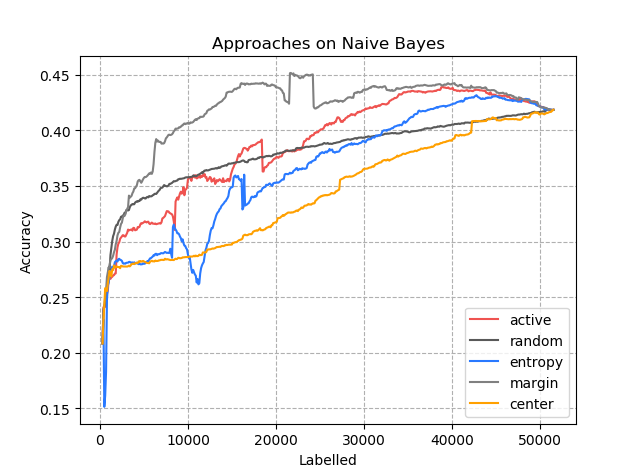
\includegraphics[width=5.5cm, angle=0]{ec1}
}
\subfigure{
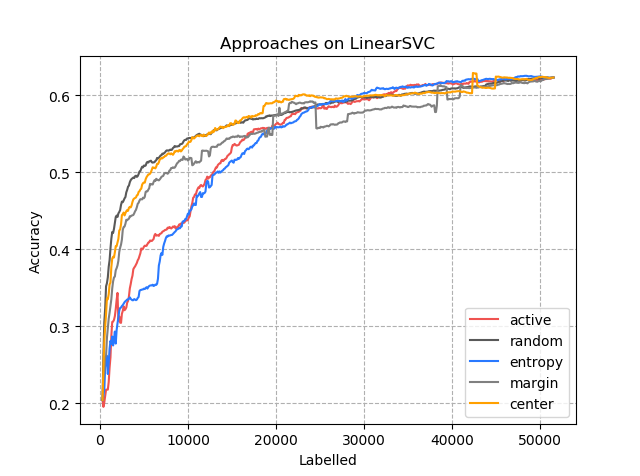
\includegraphics[width=5.5cm, angle=0]{ec2}
}
\subfigure{
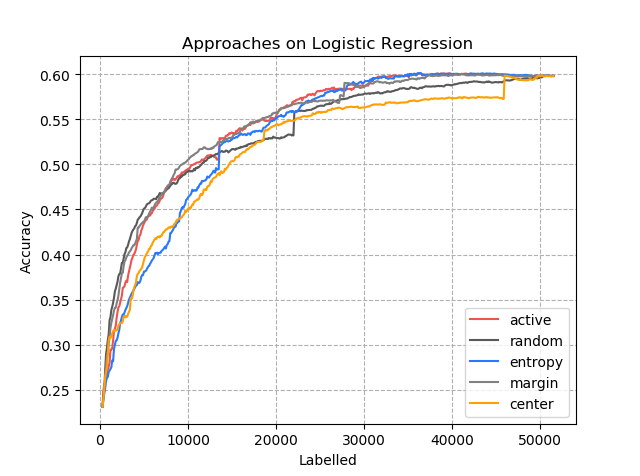
\includegraphics[width=5.5cm, angle=0]{ec3}
}
\caption{Results on E-commerce customer queries data set}
\label{fig:ec}
\end{figure*}
In this section we first describe the settings, datasets, and classifiers used for our experiments. Then, we present the results comparing the learning curves achieved with learning on different data sets and  sampling approaches.
\subsection{Classifiers}
We feed labeled data to several simple classifiers, such as Naive Bayes classifier, Support Vector Machines, logistic regression classifier.
\begin{enumerate}
    \item Naive Bayes classifiers are a family of simple \textit{probabilistic classifiers} based on applying Bayes' theorem with strong (naive) independence assumptions between the features.
    \item A Support Vector Machine model is a representation of the examples as points in space, mapped so that the examples of the separate categories are divided by a clear gap that is as wide as possible. New examples are then mapped into that same space and predicted to belong to a category based on which side of the gap they fall.
    \item Logistic regression is a statistical method for analyzing a data set in which there are one or more independent variables that determine an outcome. The outcome is measured with a dichotomous variable (in which there are only two possible outcomes).
\end{enumerate}

\subsection{Data Sets}

\begin{figure*}
\centering% Requires \usepackage{graphicx}
\begin{subfigure}
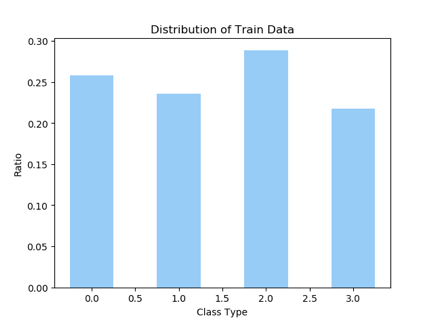
\includegraphics[width=3.3in, angle=0]{tbtrain}
\end{subfigure}
\begin{subfigure}
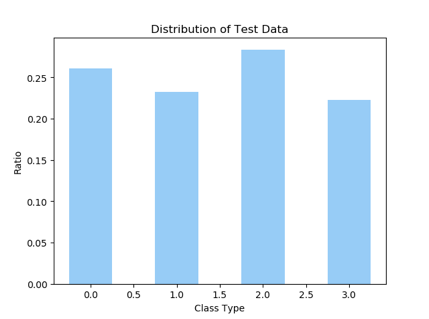
\includegraphics[width=3.3in, angle=0]{tbtest}
\end{subfigure}
\caption{Distribution of train and test data on Taobao Review}
\label{fig:tbanalysis}                
\end{figure*}

\begin{figure*}
\centering% Requires \usepackage{graphicx}
\begin{subfigure}
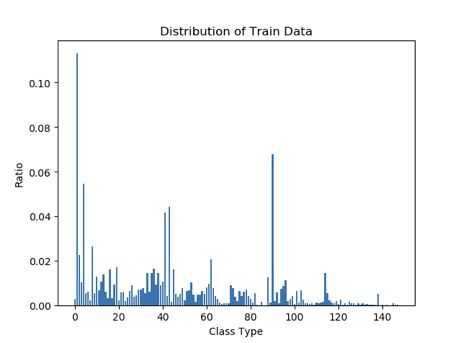
\includegraphics[width=3.3in, angle=0]{ectrain}
\end{subfigure}
\begin{subfigure}
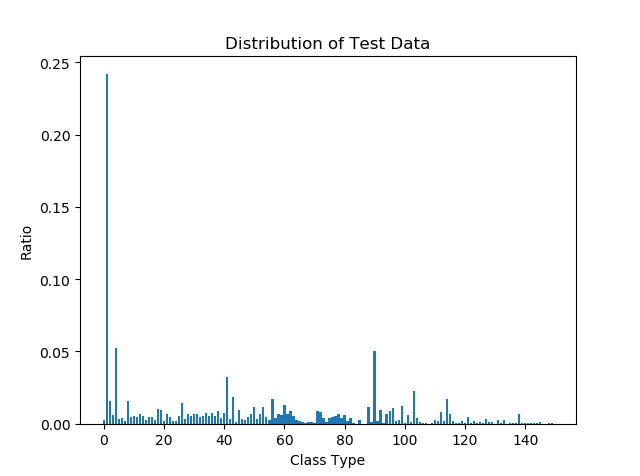
\includegraphics[width=3.3in, angle=0]{ectest}
\end{subfigure}
\caption{Distribution of train and test data on E-commerce customer queries}
\label{fig:ecanalysis}
\end{figure*}
The downstream task for our active learning algorithms is text classification. It is performed on two data sets. One is crawled Taobao reviews of different item categories, which is illustrated in Figure~\ref{fig:tbdb}. The other one is provided E-commerce customer queries of different intents, which is illustrated in Figure~\ref{fig:ecdb}. 
Different from common works, we put our emphasis on a multi-class classification tasks, which is trikier than previous works.

\subsection{Data Preprocessing}
When it comes to preprocessing procedure, we first segment our comments into words, and remove the stopwords. After that, we use our word list to calculate TF-IDF\cite{joachims1996probabilistic}.  In Word2Vec\cite{le2014distributed}, we feed the word list to get word vectors, then calculate the sentence vector by averaging all the word vectors in the sentences.
\subsection{Results}
\label{subsec:experiments}
\subsubsection{Results on Taobao Review}

Results using different classifiers  on Taobao reviews are shown in Figure~\ref{fig:tb}.  The X-axis is the amount of labelled data, while the Y-axis is the accuracy of the classifier. Since our goal is to make the decision boundary as accurate as possible using the fewest labeled points. The beginning point is the same since we set the same initial labelled data. The ending point is the same since when all the points have been sampled, it becomes a supervised problem. So we can simply evaluate the performance of different models by area under curve(AUC). The larger the area under the curve, the better the result. The red line denotes the uncertainty sampling method, the blue one is the entropy sampling approach, the gray one is the margin-based sampling, and the black one is our baseline, random sampling. From the left of Figure~\ref{fig:tb} to right, we use three different classifiers, naïve bayes, linear SVC and logistic regression. Although proposed method doesn't have a big margin over the baseline, we can expect they share some similar patterns.  For example, we can assume the gray line which is the margin-based approach is better than other methods.
\subsubsection{Results on E-commerce customer queries}



On our E-commerce customer queries, as shown in Figure~\ref{fig:ec}, from left to right we use three different classifiers, naïve bayes, linear SVC and logistic regression. Although the gray one makes a big margin over others on Naive Bayes, it performs poorly on linear SVC. In other words, it is not a consistent result. To explain this case, we do some analysis on our data.


\subsection{Analysis}

To further analyze the inconsistent results achieved on E-commerce queries, we compare its train and test data distribution with Taobao data distribution.
Figure~\ref{fig:tbanalysis} is the normalized distribution of our Taobao review data. As is shown on the figure, the distribution of the test and train data is totally the same.
However, as is shown in Figure~\ref{fig:ecanalysis}, the train data and test data of our E-commerce queries is imbalanced, which is not as ideal as Taobao review data. Nonuniformity between train data and test data may be the main reason of the inconsistency in our experiment result.
 
\section{Conclusion}
\label{sec:conclusion}
We have implemented several proposed models on our multi-class text classification tasks and also designed a procedure to improve it. Results have shown that it does work on most of the cases, but it cannot perform equally well using different classifiers on imbalanced data sets.   

To further improve our models, we have come up with some new ideas. Since previous approaches are general methods, we can go deeper and extract some features of our specific tasks. For example, we can use zero shot learning to solve the imbalanced data distribution problem. The relation between different classes, and transfer learning methods can also be used to adapt the model trained on classes with more wealthy data to classes with less data. In addition, since classifiers employed now are mainly applied in binary classification tasks, thus interfering with its performance in multi-class classification tasks. Meanwhile, they are too simple to extract higher semantic structure. Therefore, a more complicated classifier model like LSTM with attention will be leveraged to do the task.

\begin{acks}
We are grateful to the following people for resources, discussions and
suggestions: Prof. Li Jiang, Prof.
Kenny Zhu and teacher assistants Chaoqun chu and Xiaoyi Sun. We also thank E-commerce company, who provide queried labeled data.
\end{acks}

% Bibliography
\bibliographystyle{ACM-Reference-Format-Journals}
\bibliography{acmtog-sample-bibfile}
                                % Sample .bib file with references that match those in
                                % the 'Specifications Document (V1.5)' as well containing
                                % 'legacy' bibs and bibs with 'alternate codings'.
                                % Gerry Murray - March 2012


\end{document}
% End of v2-acmtog-sample.tex (March 2012) - Gerry Murray, ACM
